% KU Leuven latex poster template
%
% © 2017 Benjamin Dieudonné
%
% This work is licensed under the Creative Commons Attribution 3.0 Unported License.
% To view a copy of this license, visit
% http://creativecommons.org/licenses/by/3.0/ or send a letter to Creative
% Commons, 444 Castro Street, Suite 900, Mountain View, California, 94041, USA.

\documentclass[english,xcolor=table,t]{beamer}

% PACKAGES
\usepackage[utf8]{inputenc}
\usepackage[T1]{fontenc}
\usepackage{amsmath}
\usepackage[nolist,nohyperlinks]{acronym}
\usepackage{babel,lmodern,graphicx,mathptmx,xspace,wasysym,microtype,booktabs,tabularx,relsize,textcomp,longtable,lipsum,colortbl,eurosym,url,multicol,etoolbox,multimedia,pdfpages,fixltx2e,ifluatex,epstopdf}
\usepackage[olditem,oldenum]{paralist}
\usepackage[babel=true]{csquotes}
\usepackage[thinqspace,amssymb,textstyle]{SIunits}
\usepackage[textsize=tiny]{todonotes}
\usepackage[symbol]{footmisc}
\usepackage[notquote]{hanging}
\usepackage[normalem]{ulem}
\usepackage{changepage}
\usepackage[square]{natbib}
\input{templates/definitions.tex}

% POSTER DIMENSIONS
% header
\newcommand\posterwidth{100} % [cm]
\newcommand\posterheight{100} % [cm]
\deflen{headerheight}{15cm}
\deflen{titlemargin}{1.5cm} % margin under title
\deflen{authormargin}{1cm} % margin under authors

% blocks
\newcommand\ncol{2} % for margins
\newcommand\marginfactor{1} % for larger/smaller margin (default: 1, 0 means no margins between blocks)

% font sizes: large, Large, LARGE, huge, Huge, veryHuge, VeryHuge, VERYHuge
\setbeamerfont{title in headline}{size=\VERYHuge,series=\bfseries}
\setbeamerfont{author in headline}{size=\veryHuge}
\setbeamerfont{institute in headline}{size=\huge}

\setbeamerfont{block title}{size=\huge,series=\bfseries}
\setbeamerfont{block body}{size=\large}

\setbeamerfont{structure}{size=\LARGE} % subtitles
\setbeamerfont*{item}{parent=normal text}
\setbeamerfont{caption}{size=\large}

\setbeamerfont{itemize/enumerate subbody}{size=\large} %to set the body size

% POSTER INFO
\newcommand\postertitle{Title}
\newcommand\posterauthors{Author 1, Author 2}
\newcommand\posterinstitute{institute}

\newcommand\posterurl{university.edu}
\newcommand\posterlonginstitute{long institute name}
\newcommand\posteremail{author@university.edu}

\usepackage[size=custom,width=\posterwidth,height=\posterheight]{templates/beamerposter}

\pdfstringdefDisableCommands{\renewcommand{\sout}{}}
\graphicspath{{figures/}}
% Fix sort order in case the same file exists with multiple extensions
\DeclareGraphicsExtensions{.pdf,.png,.jpeg,.jpg,.eps}
\frenchspacing

% beamer
\mode<presentation>

% derived dimensions (logo size, margins, ...)
\newbox{\layoutbox}
\deflen{logowidth}{\headerheight}
\deflen{logoheight}{\logowidth*\ratio{236px}{661px}}
\deflen{margin}{\marginfactor\logoheight*\ratio{1px}{2px}}
\deflen{keyheight}{0.9\headerheight}
\deflen{keywidth}{\keyheight*\ratio{269px}{576px}}
\deflen{colwidth}{\paperwidth*\ratio{1px}{\ncol px}-\margin-\margin*\ratio{1px}{\ncol px}}

% colors
\setbeamercolor{background canvas}{bg=kulbg}

\setbeamercolor{headline}{fg=white,bg=kulbg}
\setbeamercolor{whitespace}{fg=white,bg=white}

\setbeamercolor{footline}{fg=white,bg=kulbg}
\setbeamerfont{footline}{size=\normalsize}

\setbeamercolor*{normal text}{fg=kullight}

\setbeamercolor*{block body}{bg=kullight,fg=kuldark}
\setbeamercolor*{block title}{bg=kullight,fg=kuldark}
\setbeamercolor*{block title example}{bg=kullight,fg=kuldark}
\setbeamercolor*{block body example}{bg=kullight,fg=kuldark}

\setbeamercolor{structure}{fg=kuldark}
\setbeamercolor*{item}{fg=kuldark}
\setbeamercolor{caption}{fg=kuldark}

\setbeamercolor{}{fg=kuldark} % e.g. figure caption

\setbeamertemplate{navigation symbols}{} % no navigation on a poster

\setbeamertemplate{headline}{%
  \begin{beamercolorbox}[ht=0.9\logoheight,wd=\paperwidth]{whitespace}%

  \end{beamercolorbox}
    \vskip-0.4\logoheight
    \leftskip0.5\logoheight
    \begin{beamercolorbox}[ht=\logoheight,wd=\logowidth]{whitespace}%
    	\includegraphics[height=\logoheight]{templates/kuleuven}  
    \end{beamercolorbox}
    
    \leftskip0ex
    \begin{beamercolorbox}[wd=\paperwidth]{headline}%
      \begin{columns}[T,totalwidth=\paperwidth]
        \begin{column}{0.9\logoheight} \end{column} % margin
        
        \begin{column}{\paperwidth-1.4\logoheight-\keywidth}
          \vskip0.5\logoheight
          {\usebeamerfont{title in headline}\postertitle \\[\titlemargin]}
          {\usebeamerfont{author in headline}\posterauthors \\[\authormargin]}
          {\usebeamerfont{institute in headline}\posterinstitute }
        \end{column}
        
        \begin{column}{\keywidth}
          \vskip-0.3\logoheight
          \raggedleft\includegraphics[height=\keyheight]{templates/key}
        \end{column}
        \begin{column}{0.5\logoheight} \end{column} % margin
      \end{columns}
    \end{beamercolorbox}
}

\setbeamertemplate{footline}{
  \begin{beamercolorbox}[ht=1.5\margin,leftskip=1.6\margin,rightskip=1.6\margin]{footline}%
    \url{\posterurl} \hfill \posterlonginstitute \hfill \texttt{\posteremail}
    \vskip 0.5\margin
  \end{beamercolorbox}
}

\setbeamertemplate{block begin}{%
\begin{beamercolorbox}[rounded=false,shadow=false]{block body}%
  \begin{beamercolorbox}[ht=0.5\logoheight,dp=0.9ex,rounded=false,shadow=false]{block title}%
     \begin{adjustwidth}{0.3\logoheight}{0.3\logoheight} 
	     \usebeamerfont*{block title}\insertblocktitle
     \end{adjustwidth}
  \end{beamercolorbox}%
  
  \begin{beamercolorbox}[ht=6pt,rounded=false,shadow=false]{block title}%
    \leftskip0.1\logoheight \rule{\textwidth-0.2\logoheight}{6pt}
  \end{beamercolorbox}%
    
  \usebeamerfont{block body}%
  \begin{beamercolorbox}[rounded=false,shadow=false,leftskip=0cm,vmode,rightskip=0cm]{block body}%
  \begin{adjustwidth}{0.3\logoheight}{0.3\logoheight}
    \parskip1em
}

\setbeamertemplate{block end}{
	\vskip0.1em 
	\end{adjustwidth}
	\end{beamercolorbox}
\end{beamercolorbox}
	  \vskip\margin
}

\setbeamertemplate{block example begin}{%
  \usebeamerfont{block body}%
  \begin{beamercolorbox}[rounded=false,shadow=false,leftskip=0cm,vmode,rightskip=0cm]{block body example}%
  \begin{adjustwidth}{0.3\logoheight}{0.3\logoheight}
    \parskip1em
}

\setbeamertemplate{block example end}{
	\vskip0.1em 
	\end{adjustwidth}
	\end{beamercolorbox}
	  \vskip\margin
}

%\setbeamertemplate{structure text begin}{\vskip.4em}

\setbeamertemplate{itemize/enumerate body begin}{
\begin{minipage}{\dimexpr\textwidth-0.3\logoheight}
\begin{adjustwidth}{0px}{0.3\logoheight} 
}

\setbeamertemplate{itemize/enumerate body end}{
\end{adjustwidth}
\end{minipage}
}

\setbeamertemplate{itemize items}[square]

\setbeamertemplate{bibliography item}{\hskip\dimexpr0.5em+0.8cm\relax}

\setbeamertemplate{caption}{%
	\usebeamercolor[fg]{caption name}%
	\usebeamerfont*{caption name}%
	\insertcaptionname~\insertcaptionnumber:~%
	\insertcaption\par
}

\newenvironment{vfillcolumn}[1]{%
\begin{column}{#1}
\minipage[c][\textheight][s]{#1}
\vskip \margin
}{%
\endminipage
\end{column}
} % all formatting is defined here

% POSTER CONTENT
\begin{document}
\begin{frame}
\begin{columns}
\begin{vfillcolumn}{\colwidth}
\begin{block}{First block}
Lorem ipsum dolor sit amet, consectetur adipiscing elit. Proin pharetra facilisis nisi ac lacinia. Quisque eu dui at orci pulvinar eleifend. Etiam tempus magna eu nulla fringilla cursus. Nunc augue leo, porta eget fermentum ultricies, varius quis ex. Aliquam consequat odio sed nulla fringilla, sed porta nunc rhoncus. Maecenas et sem orci.

\blocksubtitle{A subtitle}
In a est vitae orci sodales laoreet. Mauris ultricies, sapien at porta semper, purus dui fermentum libero, in gravida risus justo eu felis. In nec pretium nisi. Pellentesque sed nisl sed ligula varius pharetra et id felis. In a maximus elit. Sed non consectetur sem, ac ornare libero. Aliquam ut tellus efficitur, fringilla felis id, euismod nisl.
\end{block}

\vfill
\begin{block}{Enumerate and itemize block}
\begin{itemize}
\item Lorem ipsum dolor sit amet, consectetur adipiscing elit. Proin pharetra facilisis nisi ac lacinia. Quisque eu dui at orci pulvinar eleifend. 

\item Etiam tempus magna eu nulla fringilla cursus. 
\begin{itemize}
\item Nunc augue leo,
\item porta eget fermentum ultricies, varius quis ex. 
\end{itemize}
\end{itemize}

\begin{enumerate}
\item Lorem ipsum dolor sit amet, consectetur adipiscing elit. Proin pharetra facilisis nisi ac lacinia. Quisque eu dui at orci pulvinar eleifend. 

\item Etiam tempus magna eu nulla fringilla cursus. 
\begin{enumerate}
\item Nunc augue leo,
\item porta eget fermentum ultricies, varius quis ex. 
\end{enumerate}
\end{enumerate}

\end{block}

\vfill
\begin{block}{Another block}
Lorem ipsum dolor sit amet, consectetur adipiscing elit. Proin pharetra facilisis nisi ac lacinia. Quisque eu dui at orci pulvinar eleifend. Etiam tempus magna eu nulla fringilla cursus. Nunc augue leo, porta eget fermentum ultricies, varius quis ex. Aliquam consequat odio sed nulla fringilla, sed porta nunc rhoncus. Maecenas et sem orci. In a est vitae orci sodales laoreet. Mauris ultricies, sapien at porta semper, purus dui fermentum libero, in gravida risus justo eu felis. In nec pretium nisi. Pellentesque sed nisl sed ligula varius pharetra et id felis. In a maximus elit. Sed non consectetur sem, ac ornare libero. Aliquam ut tellus efficitur, fringilla felis id, euismod nisl.
\end{block}

\vfill
\begin{block}{Another block}
Lorem ipsum dolor sit amet, consectetur adipiscing elit. Proin pharetra facilisis nisi ac lacinia. Quisque eu dui at orci pulvinar eleifend. Etiam tempus magna eu nulla fringilla cursus. Nunc augue leo, porta eget fermentum ultricies, varius quis ex. Aliquam consequat odio sed nulla fringilla, sed porta nunc rhoncus. 
\end{block}

\end{vfillcolumn}

\begin{vfillcolumn}{\colwidth}

\begin{exampleblock}{This title is not shown}
Block without title \citep{einstein1905elektrodynamik}.

\blocksubtitle{But it has a subtitle}
And a horizontal rule.
\blockhrule
Maecenas et sem orci. In a est vitae orci sodales laoreet. Mauris ultricies, sapien at porta semper, purus dui fermentum libero, in gravida risus justo eu felis. In nec pretium nisi. Pellentesque sed nisl sed ligula varius pharetra et id felis. In a maximus elit. Sed non consectetur sem, ac ornare libero. Aliquam ut tellus efficitur, fringilla felis id, euismod nisl.
\end{exampleblock} 

\vfill 
\begin{block}{Picture block}
\begin{figure}
	\centering
    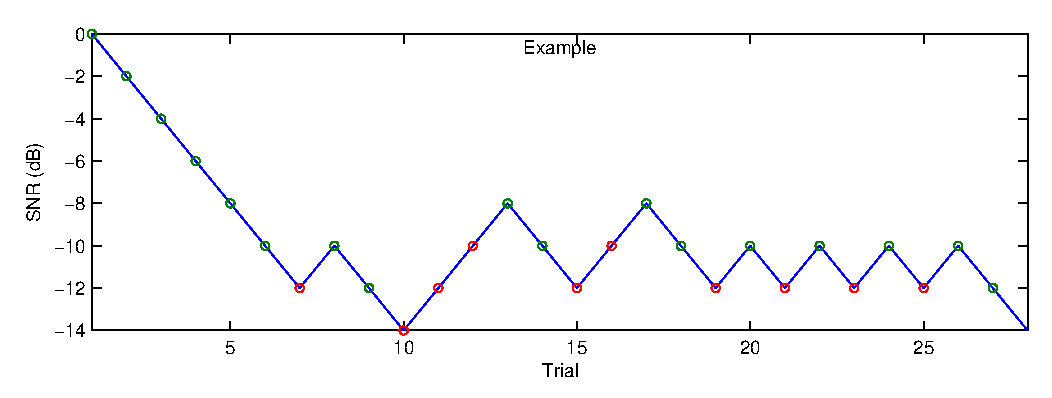
\includegraphics[width=0.5\textwidth]{presentation-examplefig}
	\caption{A picture.}
\end{figure}

\end{block}

\vfill 
\begin{block}{Picture block}
\begin{figure}
	\centering
    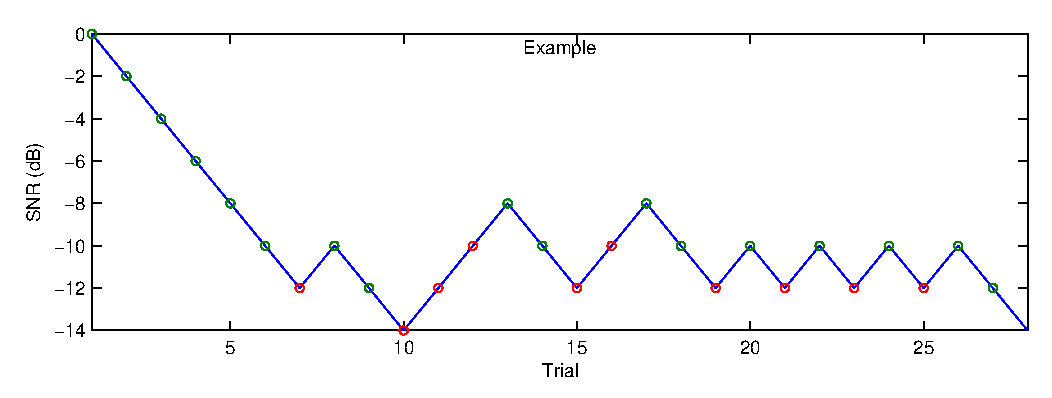
\includegraphics[width=0.5\textwidth]{presentation-examplefig}
	\caption{A picture.}
\end{figure}

\end{block}

\vfill

\begin{minipage}{0.75\colwidth}

\begin{exampleblock}{}
% ACKNOWLEDGMENTS
\vskip 3cm
Thank you all!

\vskip 3cm

\blockhrule

% REFERENCES
\vskip 3cm
\bibliographystyle{ieeetr}
\bibliography{references}

\vskip 3cm
\end{exampleblock}

\end{minipage}

\begin{exampleblock}{}
\vskip -3cm
\end{exampleblock}

\end{vfillcolumn}
\end{columns}

\vskip -16cm
      \begin{columns}[T,totalwidth=\paperwidth]
        \begin{column}{\paperwidth-0.25\colwidth-\margin} \end{column} % margin
        
        \begin{column}{0.25\colwidth}
          \centering
          \Large \textbf{DOWNLOAD \\ POSTER} \vskip 2cm
          \includegraphics[width=0.2\colwidth]{qrcode}
        \end{column}
        \begin{column}{\margin} \end{column} % margin
      \end{columns}
\end{frame}
\end{document}
